\documentclass[pdf]{beamer}
\usepackage{caption}

\title{Modeling of spin-orbital dynamics in a storage ring}

\begin{document}
	\begin{frame}
		\titlepage
	\end{frame}	

	\begin{frame}
		\frametitle{Tasks from supervisor}
		\begin{itemize}
			\item Study effects of WF tilts (preserves Lorentz force) in FS lattice on $S_x, S_y, S_z$;
			\item Same for quadrupole shifts (doesn't preserve LF);
			\item Study decoherence as a function of the inital beam distribution ($x, y, \delta W$);
			\item Study optimal sextupole placement for the suppression of decoherence and chromaticity;
			\item Modeling of field calibration by effective gamma in the horizontal plane (CW/CCW procedure);
		\end{itemize}
	\end{frame}

	\begin{frame}
		\frametitle{Conventional ODE integrator}
		\framesubtitle{Python prototype}
		\begin{itemize}
			\item Wrote that fbecause couldn't get COSY INFINITY to produce results that I could interpret;
			\item Classes defining most commonly utilized accelerator elements (dipoles, quadrupoles, Wien filters, etc);
			\item Two versions of element positioning imperfections (tilting):
			\begin{itemize}
				\item via computing the tilt matrix, and applying it to the computed field at run time (more general but time-consuming, doesn't preserve guiding field strength by default);
				\item customized tilting for dipole, WF (less time-consuming, preserves the Lorentz force acting on the particle), and shift for quadrupole;
			\end{itemize}
		\item Vectorized RHS computation.
		\end{itemize}
	\end{frame}

	\begin{frame}
		\frametitle{Example plots}
		\begin{columns}
			\column{.5\textwidth}
			\begin{itemize}
				\item $S_x \sim s$ in FS lattice w/o tilt
				\item $S_x \sim s$ in FS structure w/ all elements tilted about $\hat s$
				\item $S_y \sim s$ in FS structure w/ elements randomly tilted Norm(0, $10^{-4}$ rad)
			\end{itemize}
			\begin{minipage}{.3\textheight}
				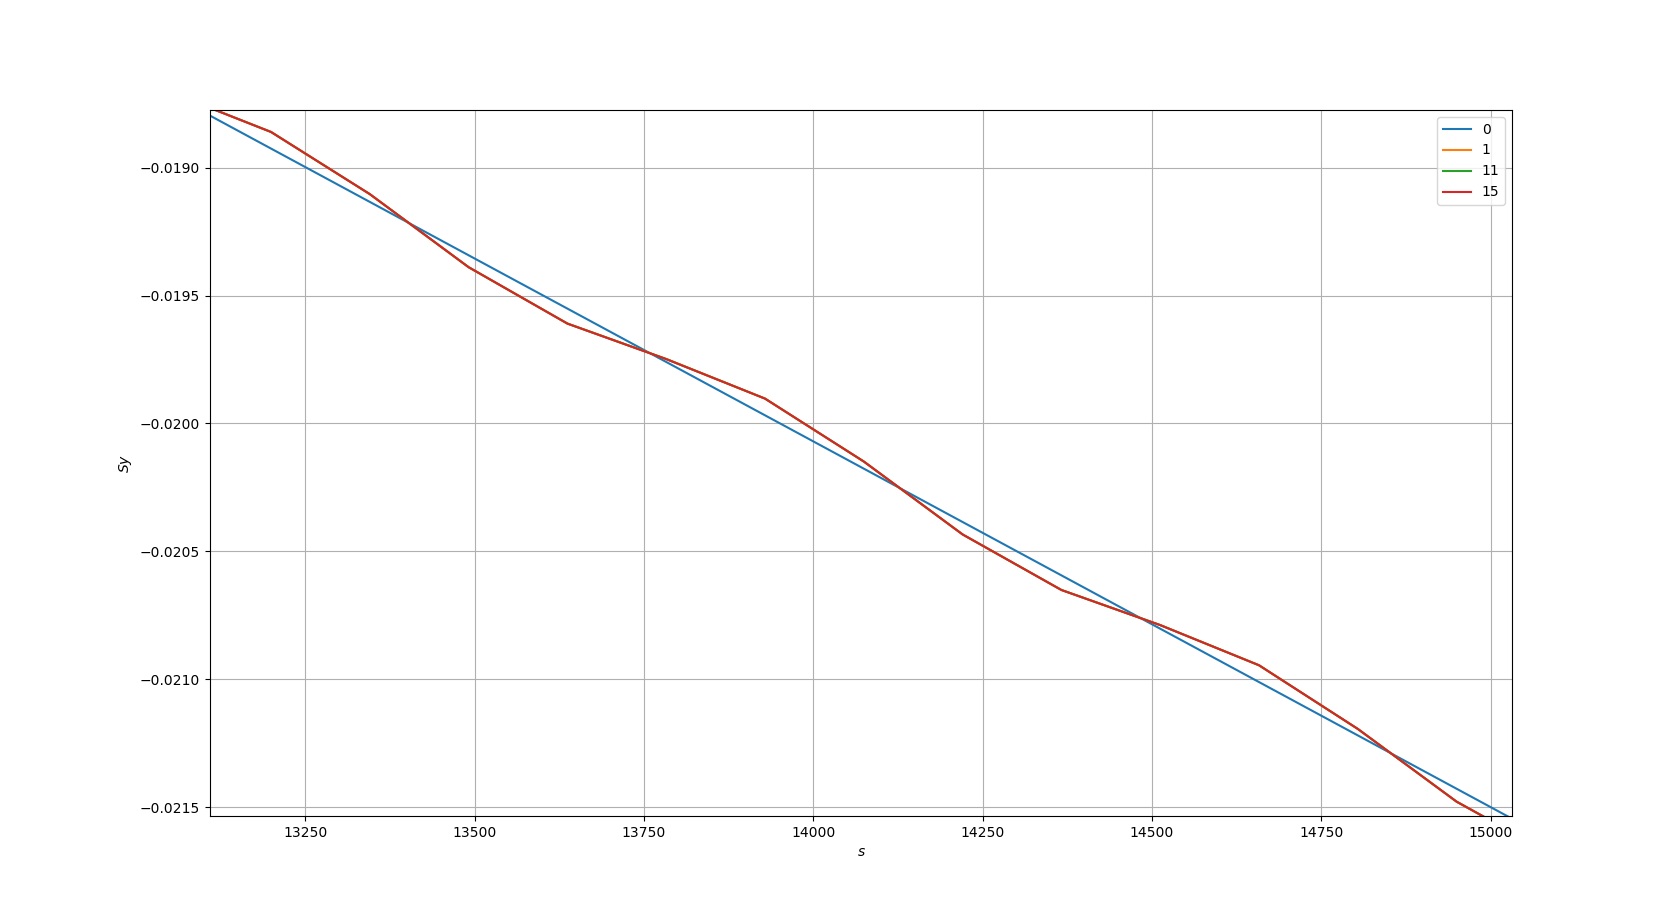
\includegraphics[scale=.15]{Sy_300_sigma_tilts_0057_deg_piece}
			\end{minipage}
			\column{.5\textwidth}
			\begin{minipage}{.3\textheight}
				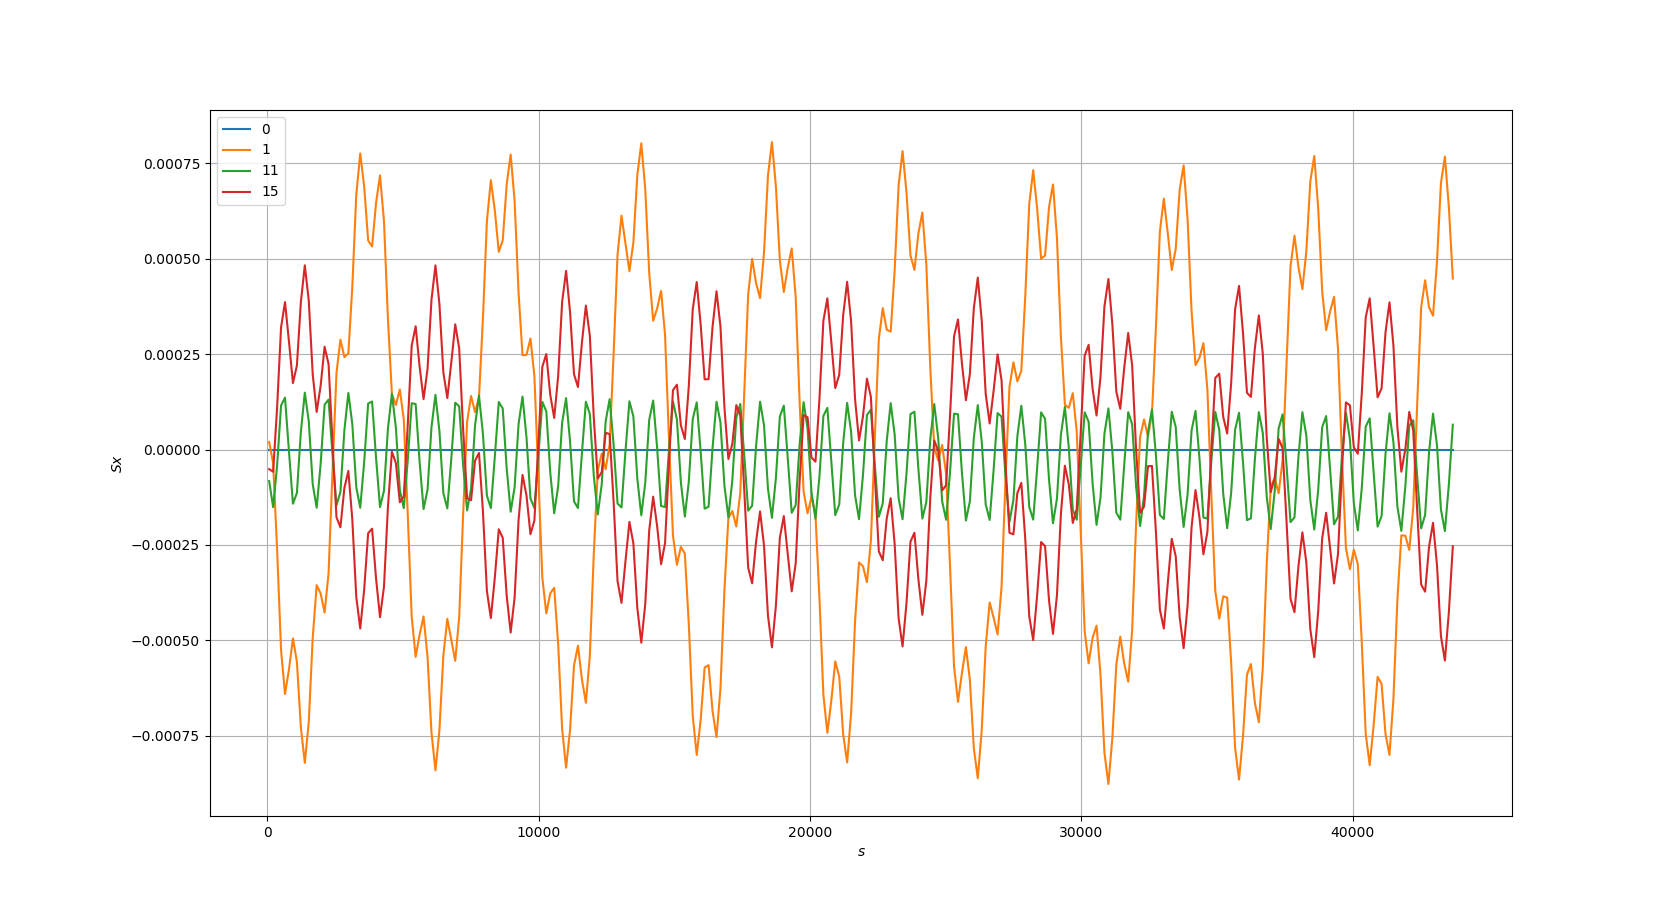
\includegraphics[scale=.15]{Sx_300_no_tilt}
			\end{minipage}
			\begin{minipage}{.3\textheight}
				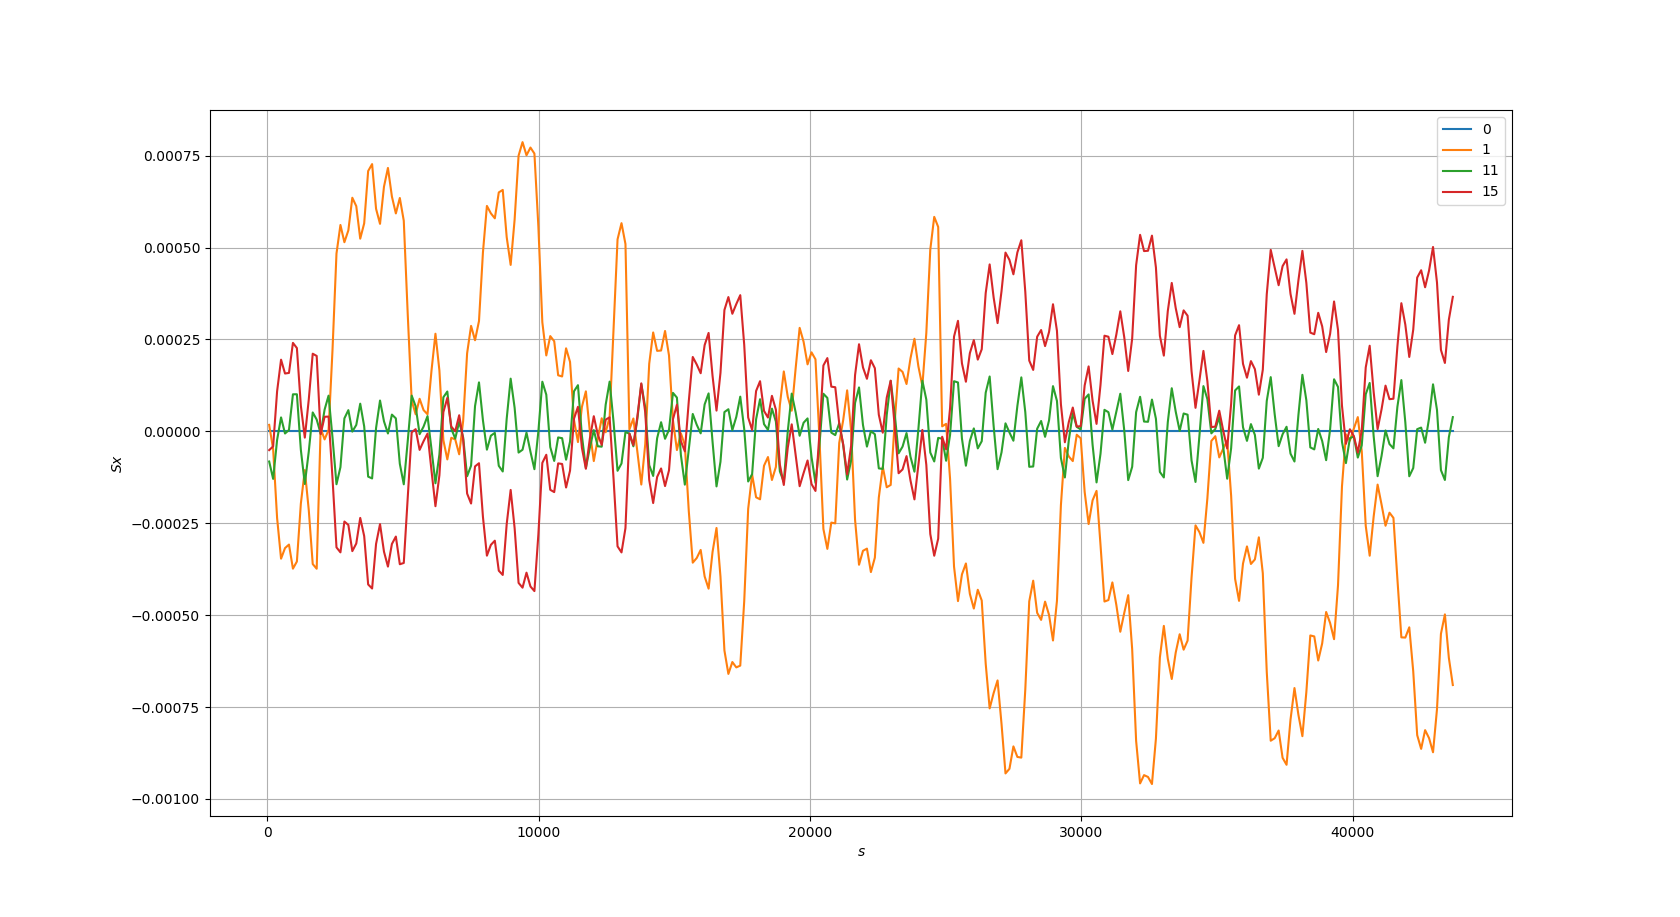
\includegraphics[scale=.15]{Sx_300_all_tilts_3_6}
			\end{minipage}
		\end{columns}
	\end{frame}

%	\begin{frame}
%		\frametitle{Decoherence test histograms}
%		\begin{itemize}
%			\item 100 turns; 70 trials; 20-particle bunches: $x \sim N(0, 10^{-3})$, $y \sim N(0, 10^{-3})$, $dK \sim N(0, 10^{-4})$
%		\end{itemize}
%		\begin{figure}
%			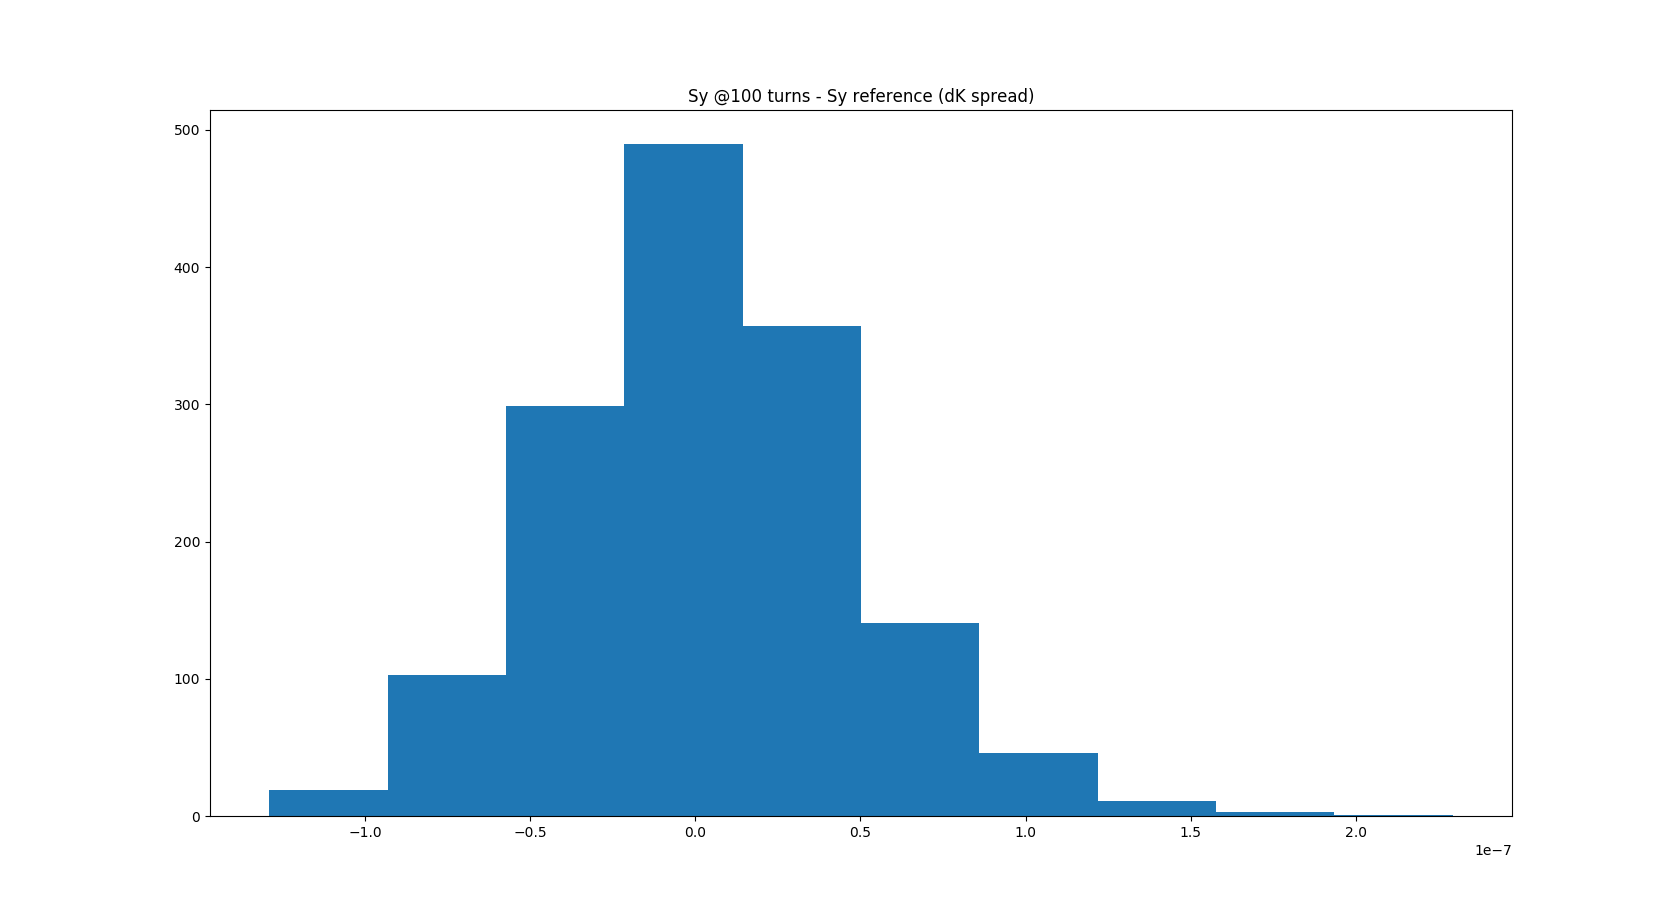
\includegraphics[scale=.25]{Sy_hist_dK}
%			\caption{Histogram from $dK \sim N(0, 10^{-4})$ test}
%		\end{figure}
%	\end{frame}
%	\begin{frame}
%		\begin{figure}
%			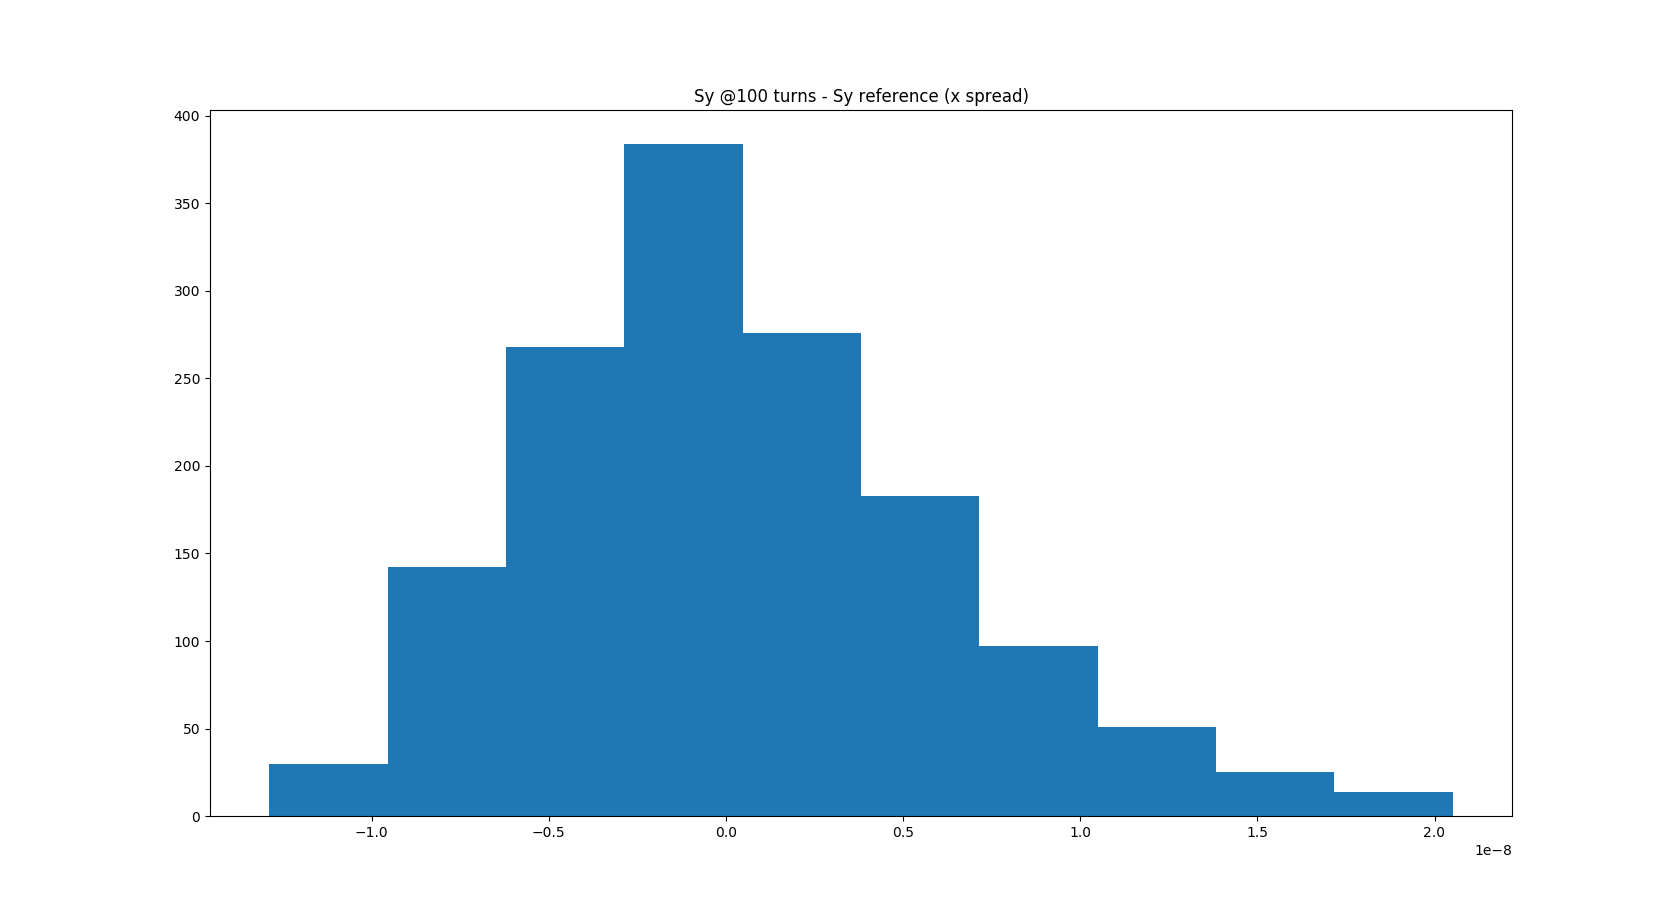
\includegraphics[scale=.3]{Sy_hist_x}
%			\caption{Histogram from $x \sim N(0, 10^{-3})$ test}
%		\end{figure}
%	\end{frame}
%	\begin{frame}
%		\begin{figure}
%			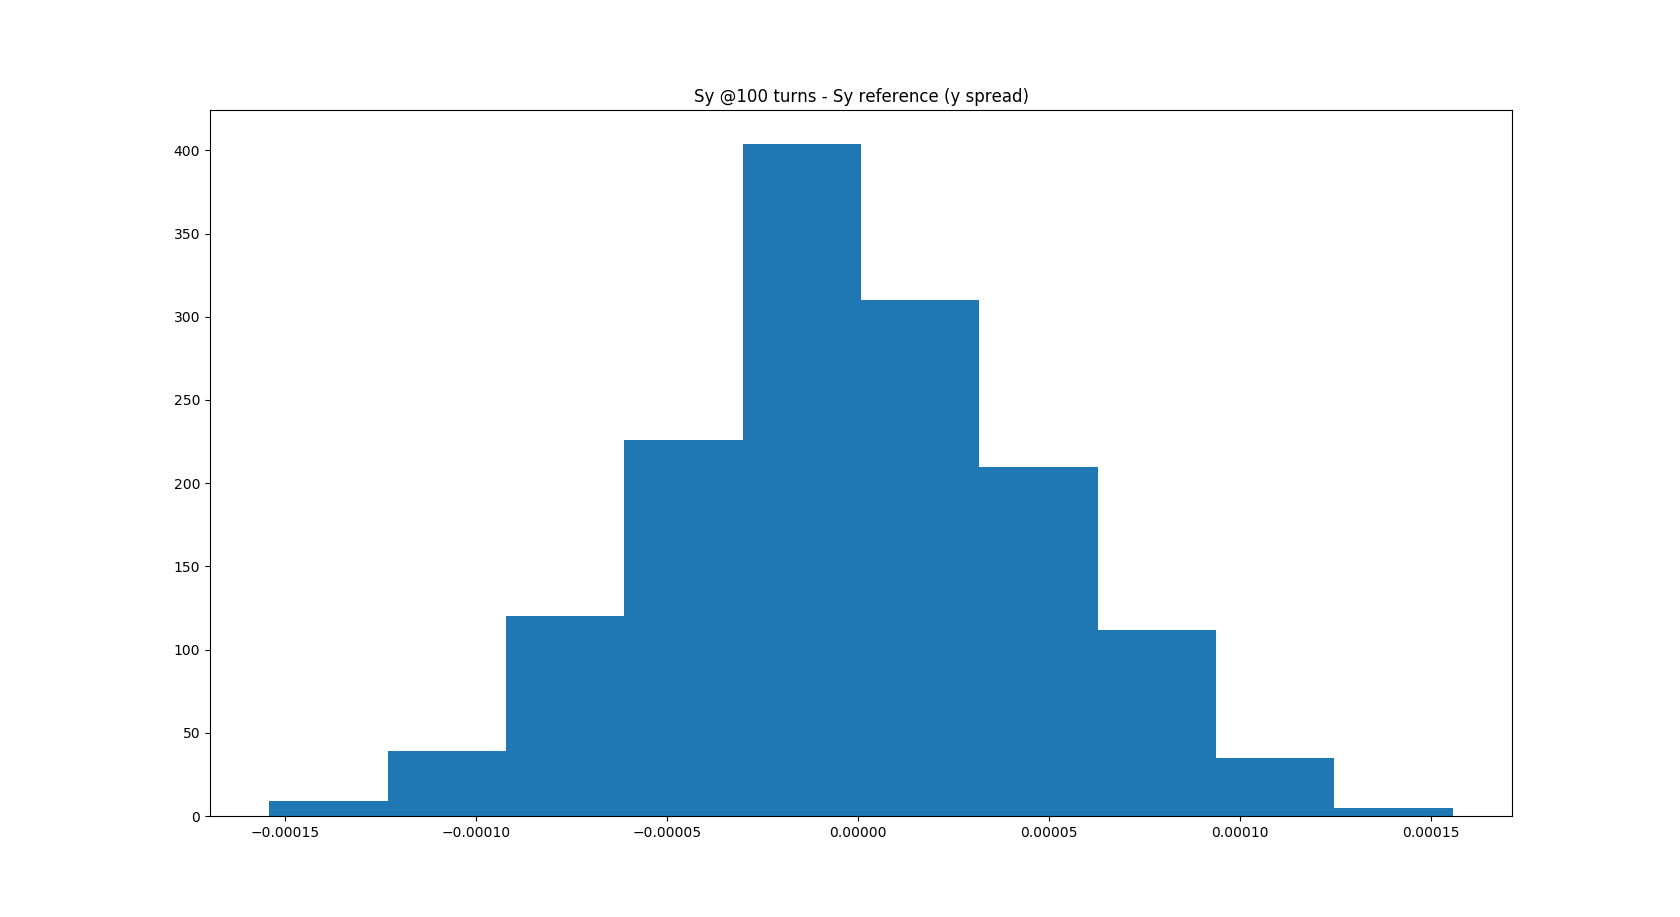
\includegraphics[scale=.3]{Sy_hist_y}
%			\caption{Histogram from $y \sim N(0, 10^{-3})$ test}
%		\end{figure}
%	\end{frame}

	\begin{frame}
		\frametitle{Conventional ODE integrator}
		\framesubtitle{C++ extension}
			\begin{itemize}
				\item $\omega_i = \omega_0 + G_6\cdot\Delta\gamma_i^2$, where $\Delta\gamma_i^2$ is the average gamma in phase space, due to synchrotron oscillations.
				\item $Q_s = \frac{\omega_s}{\omega_{rev}} \ll 1$ (like 1/35) $=>$ require thousands of turns.
				\item Reimplemented core functionality in c++
			\end{itemize}
		\centering
		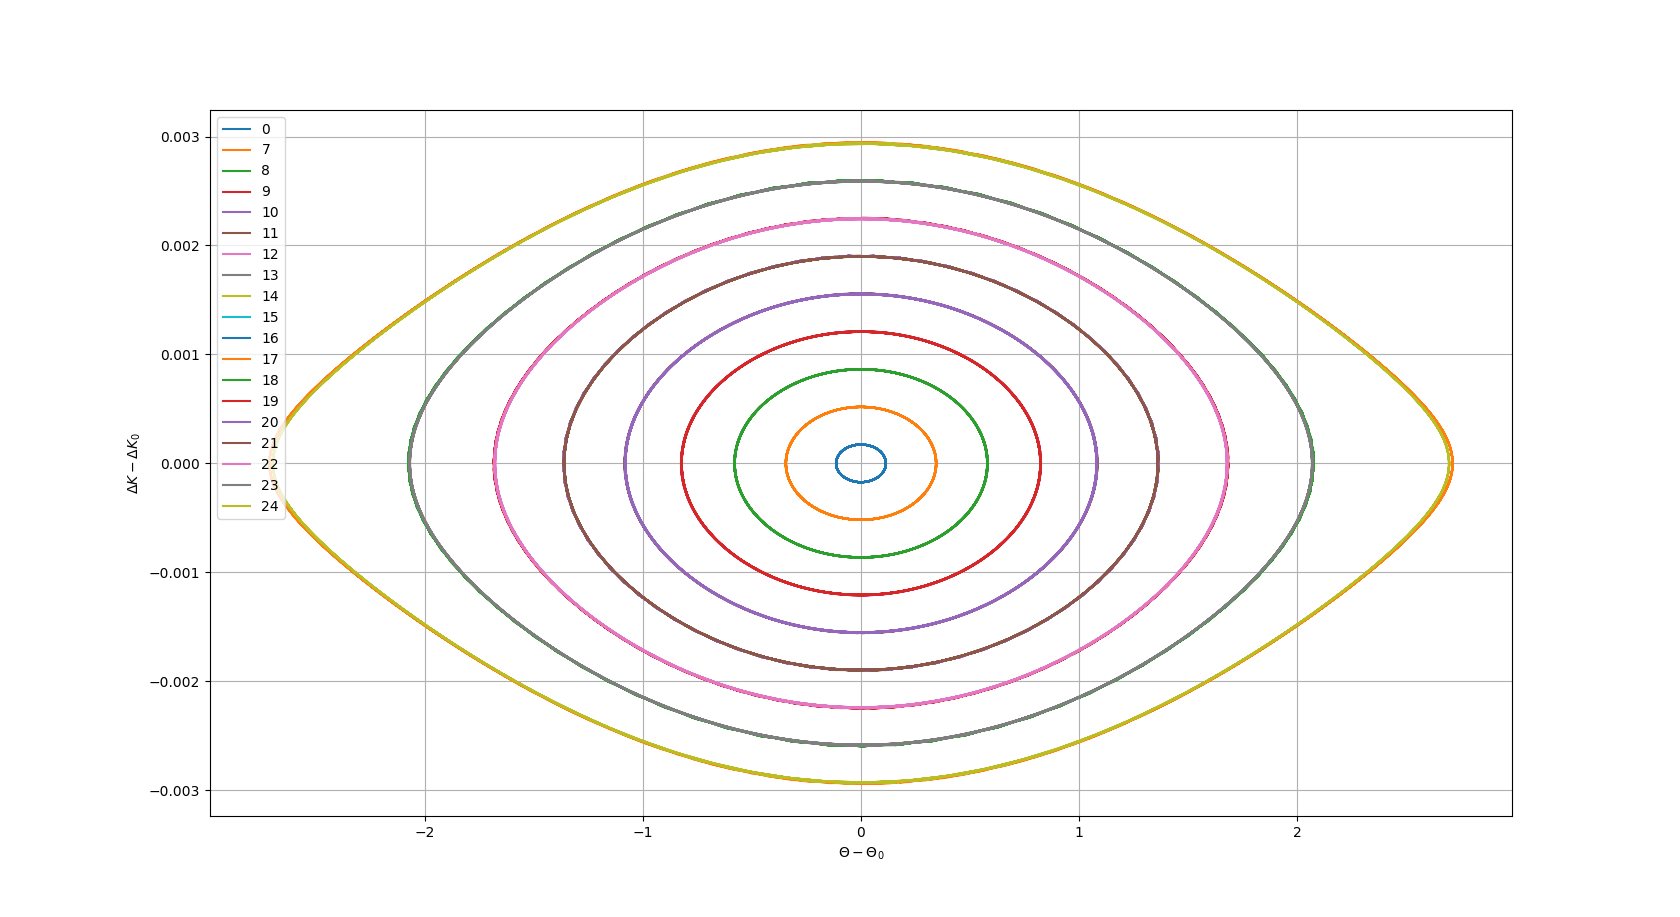
\includegraphics[scale=.25]{mean_dK_test_fishplot}
	\end{frame}
	\begin{frame}
		\centering
		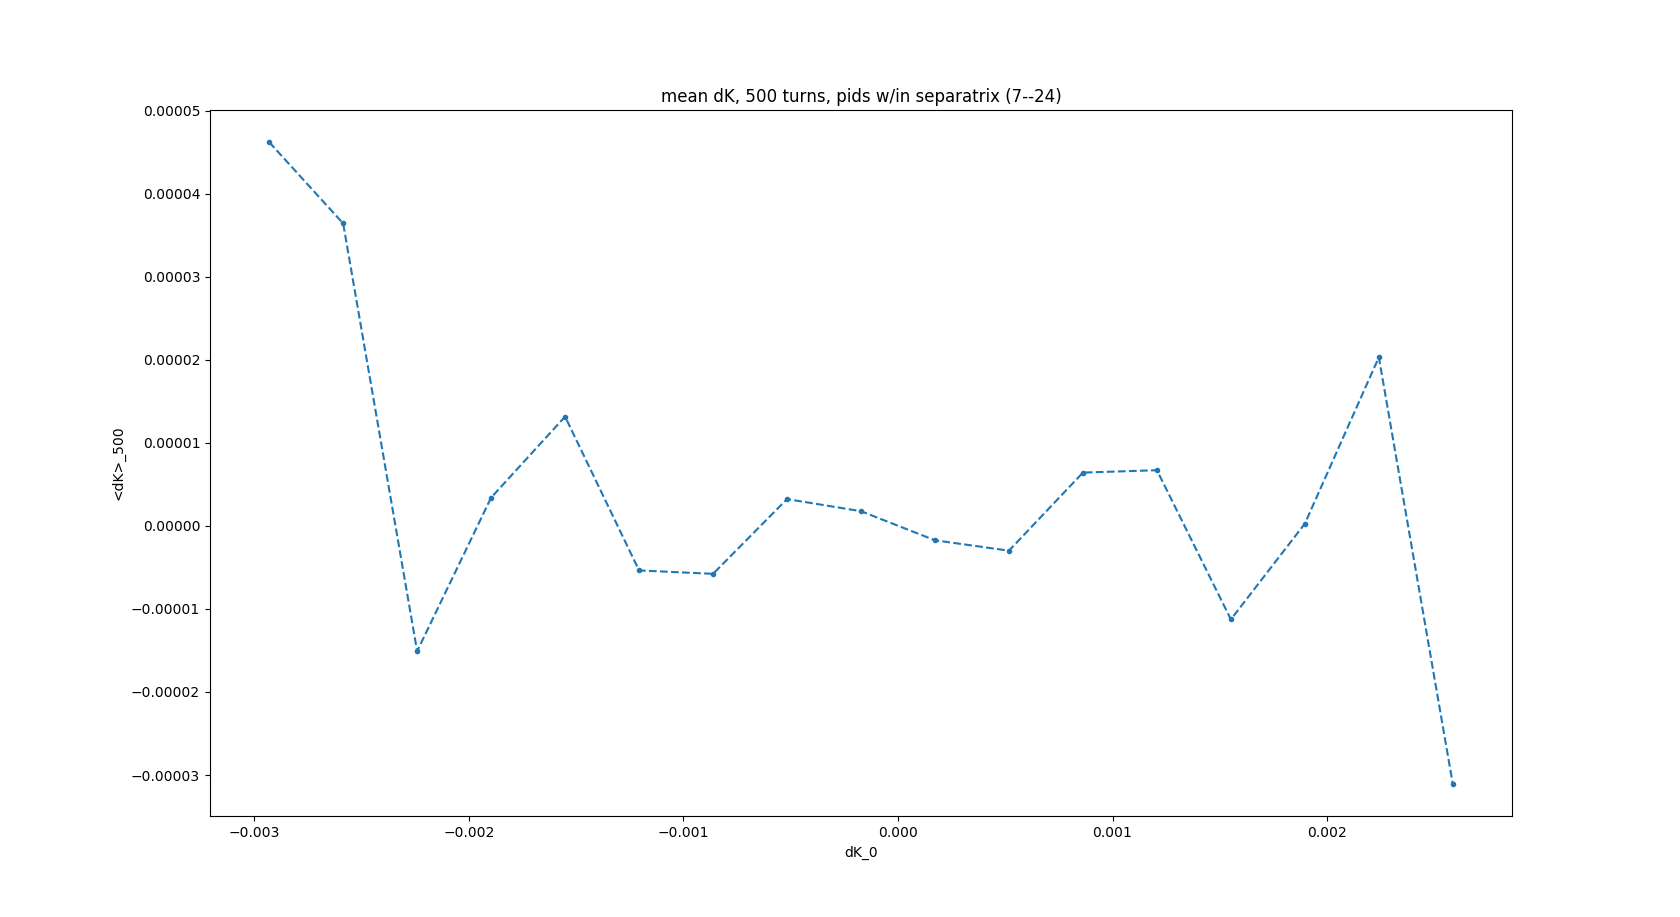
\includegraphics[scale=.3]{mean_dK_test_mean_dK_vs_dK0}
		\captionof{figure}{$\langle \Delta K\rangle$ vs $\Delta K_0$ after 500 turns (14 synchrotron oscillations)}
	\end{frame}
\begin{frame}
	\centering
	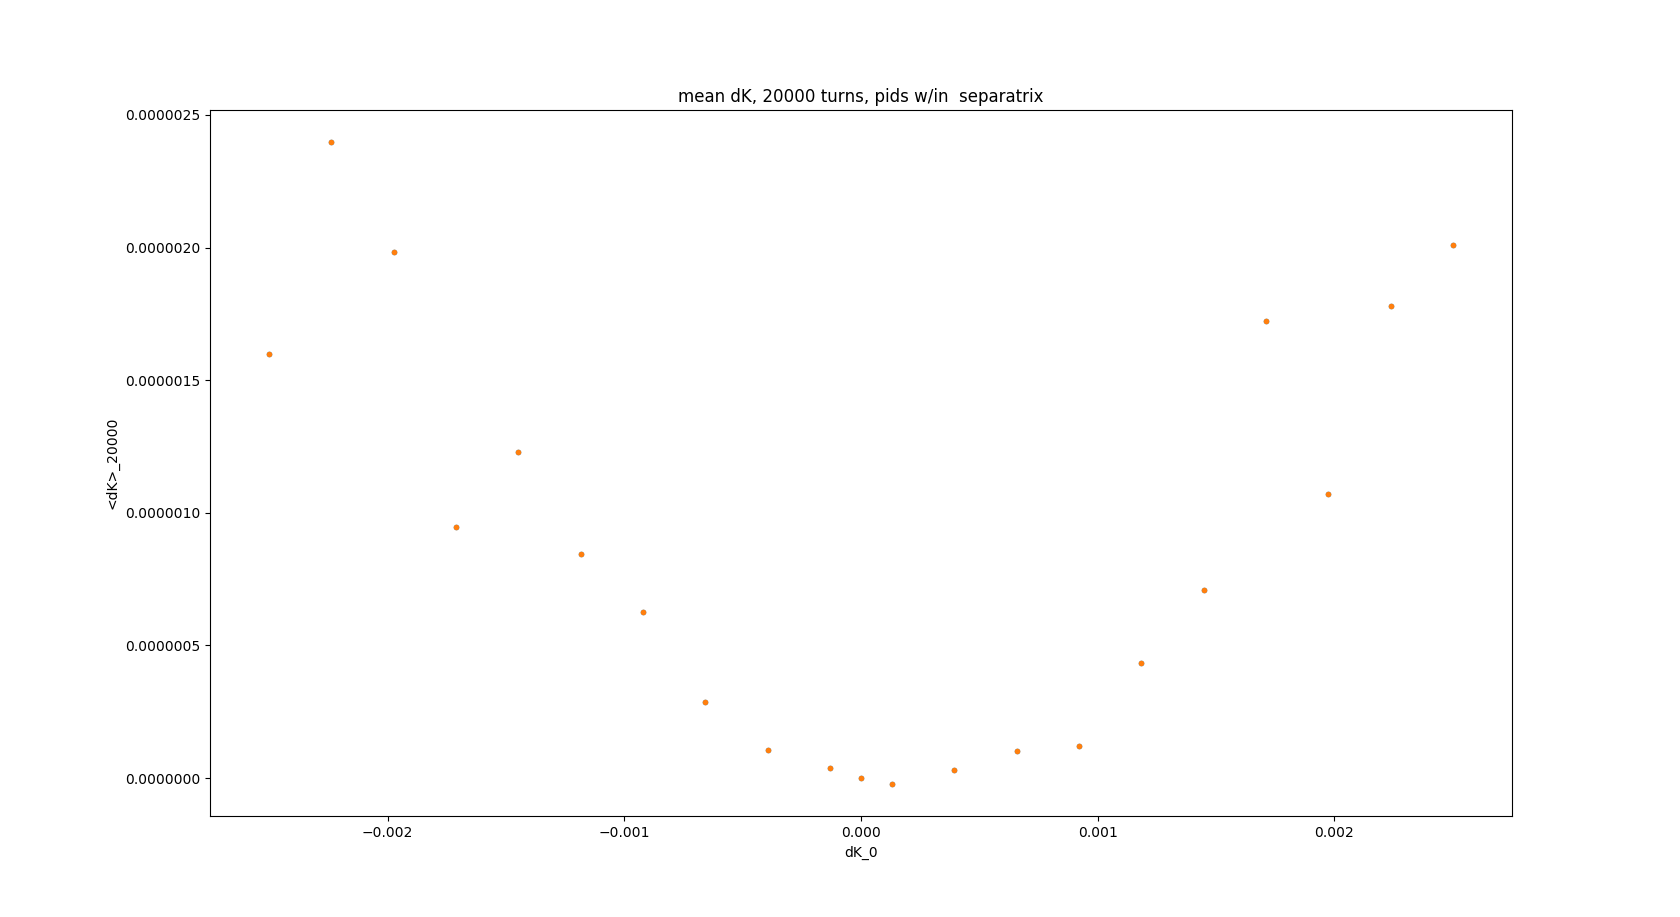
\includegraphics[scale=.3]{mean_dK_test_mean_dK_vs_dK0_20000trns_parabola}
	\captionof{figure}{$\langle \Delta K\rangle$ vs $\Delta K_0$ after 20,000 turns (571 synchrotron oscillations)}
\end{frame}
	
	\begin{frame}{Problems}
	\begin{itemize}
		\item Assuming
	\end{itemize}
	\end{frame}

\end{document}
